\section{Design of a policy matching algorithm for generating data access agreements}
\label{sec:algorithm}

In this Section, a detailed overview is given of the proposed algorithms for offer instantiation and policy matching towards the generation of a common data access agreement.
Moreover, a policy editor to define and store OAC policies in Solid Pods is described, as well as a REST API service that uses the results of the policy matching algorithm to facilitate the exercising of data subject rights.

\subsection{Development of an OAC policy editor}
\label{sec:sope}

This Section features an ODRL editor designed to define and save RDF policies, to enable the granting of access to personal data stored in Solid Pods.
RDF policies are articulated using the OAC specification developed in Section~\ref{sec:oac}.
As such, with such an OAC editor, data subjects can create intricate, detailed policies that adhere to GDPR stipulations concerning personal data processing without the burden of knowing ODRL or even RDF.

\paragraph{SOPE -- the Solid ODRL access control Policies Editor}
SOPE is a Solid-based app for data subjects to define and store ODRL policies, based on the OAC specification, on Solid Pods.
Detailed instructions on how to install, launch, and use the app are available on the source code repository\footnote{\url{https://w3id.org/people/besteves/sope/repo}}.
To use it, data subjects must already be in the possession of a Solid Pod and a WebID to be able to log into their Pod and store policies there, using SOPE.
Once logged in, users can select the type of policy they want to model, as well as choose the types of personal data and purposes to which the policy applies.
Additionally, users can also select what type of access they which to provide for said data type and purpose, as well as model further constraints, such as types of recipients that can receive the results of the personal data processing or identity providers used by data requesters to authenticate.
Finally, the prototype interface allows users to generate and store the ODRL policy's RDF in the Pod, without the need for users to be knowledgeable about OAC, ODRL, or DPV.
SOPE also stores policy logs and updates the policy registry in the user's Pod, using the PLASMA vocabulary to model such information, however, in the future, such documentation should be generated by the server to ensure interoperability (by not depending on the app's own implementation, which could diverge from app to app).
All generated information, e.g., policies, logs, and registry, is stored in a private location within the Pod -- only authorised users, apps, or services will have access to it if desired by the data subject.
Figure~\ref{fig:sope-ui} presents a screenshot of SOPE's interface.

\begin{figure}[ht]
    \centering
    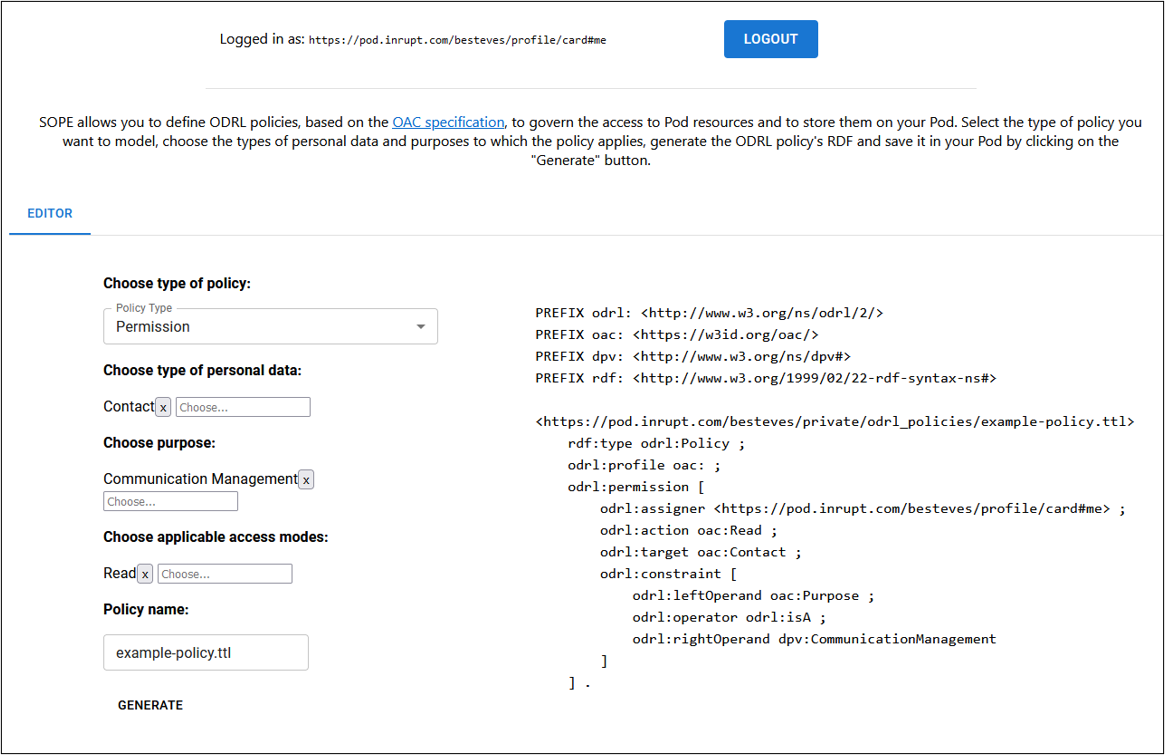
\includegraphics[width=0.9\linewidth]{figures//chapter-6/sope-snap.png}
    \caption{Screenshot of SOPE, a Solid app for editing OAC-based policies.}
    \label{fig:sope-ui}
\end{figure}

\paragraph{SOPE coverage, maintenance, and future work}
SOPE is published and archived according to the methodology described in Section~\ref{sec:code_preservation}.
Furthermore, SOPE's source code is hosted at \url{https://w3id.org/people/besteves/sope/repo}, under the CC-BY-4.0 license.
A live demonstration of the app's features is also available at \url{https://w3id.org/people/besteves/demo/eswc22}.
The repository can also be used by SOPE users to suggest new features to be added to the app and to report bugs through GitHub Issues.
%\beatriz{Table XX } illustrates the current coverage of SOPE concerning the terms implemented in the app from DPV's taxonomies of purposes, personal data categories, processing operations, and recipients.
Currently, SOPE's app coverage encloses terms from DPV's taxonomies of purposes, personal data categories, processing operations, and recipients.
As future work, SOPE can be extended to include all terms present in the previously mentioned DPV's taxonomies, as well as to cover all constraints defined in the OAC profile, e.g., restrict legal bases or specify the technical and organisational measures used by data controllers to ensure the secure processing of personal data.
Moreover, with such an extension, SOPE could also be used by data controllers to detail their privacy policies.
Additionally, user studies should be performed to assess the design choices included in the editor, as well as to understand what type of additional controls people want to have on top of what is legally mandated, e.g., temporal constraints or duties for the data controller to fulfil prior to data access.

\subsection{Data subject policies as \texttt{odrl:Offer}s}
\label{sec:algorithm-offer}

Data subjects can express policies for specific resources, containers of resources, specific personal data types, or even for data they have not produced yet.
As such, at the time of instantiation, the incoming data request should be used to filter the data subject's policies that apply to that particular request.
This is to ensure that only the needed policies are shared and no more, aligned with the `data minimisation' principle in GDPR's Article 5.1(c) \citeyearpar{noauthor_regulation_2016}, as user policies should also be considered personal data and be treated as such.
Therefore, the resulting \texttt{odrl:Offer} instance contains the union of all pertinent user policies, which can be used to match against incoming data requests in order to generate data access agreements for certain resources or data.
Furthermore, this policy can be used as metadata that accompanies the data being accessed/shared, so that data controllers can keep a copy of the conditions under which they can use the data.
In essence, such a system improves trust and accountability in decentralised data-sharing ecosystems as the policy can travel with the data, with provenance information on who generated the data, who generated the policy, and who attached it to the data.
Even though malicious agents can perform prohibited actions, such as making copies of data when only read-access to data was allowed, with the documentation of access conditions being stored on the datastore of the data subjects, they can use these policies and metadata to file a complaint in the court of law for data misuse.
Moreover, when formulating offers, each distinct rule merged into the policy is preserved as an individual rule to facilitate the matching with data requests.
This preservation of individual rules also enables their individual annotation with provenance metadata, e.g., their origin or whether they are negotiable or non-negotiable rules.

Taking this into consideration, the instantiation of the \texttt{odrl:Offer} should follow the subsequent algorithm:
\begin{enumerate}
    \item For a given personal datastore, retrieve all user preferences and requirements recorded in a datastore policy registry.
    \item Filter out duplicated policies.
    \item Filter out policies that do not match with any terms of the data request.
    \item For each retrieved policy, fetch relevant \texttt{odrl:Permission} and \texttt{odrl:Prohibition} rules and merge them in a single \texttt{odrl:Offer}.
    \item Permissions and/or prohibitions associated with an OAC requirement or an OAC preference should be associated with the term \texttt{dpv:Required}, in case said rule is a requirement, or the term \texttt{dpv:Optional}, in case it is a preference, using the \texttt{dpv:hasContext} property.
    \item A link to each `original' policy is maintained in the final \texttt{odrl:Offer} by using the \texttt{dcterms:source} property.
    \item Add provenance information to the \texttt{odrl:Offer}, e.g. \texttt{dcterms:issued} for when the offer was instantiated and \texttt{dcterms:creator} for the issuer of the policy.
\end{enumerate}

The previously described Listing~\ref{list:oac_offer} presents an example of a result of the offer instantiation algorithm, generated from two existing, relevant policies, as indicated by the \texttt{dcterms:source} property, based on an OAC requirement and OAC preference policies, as expressed by the \texttt{dpv:hasContext} property.

\subsection{Policy matching outcomes as \texttt{odrl:Agreement}s}
\label{sec:algorithm-agreement}

As mentioned in the previous Sections, the instantiated user policies are one of the few bits, representing the will of the data subject, that must be fed to the policy matching algorithm to generate the data access conditions to certain data or resources.
In addition to those, data request policies, expressing the needs and purposes of the data requesters, as well as other contextual information, e.g., date or time of the day, must also be passed on to the algorithm in order to reach a data access agreement that benefits and satisfies both parties.

The recorded outcomes, resulting from the matching process where access to data needs to be either permitted or prohibited, are instances of \texttt{odrl:Agreement}.
Within these agreements, specific ODRL terms play a crucial role in specifying who has granted or denied access (\texttt{odrl:assigner}), to whom (\texttt{odrl:assignee}), for what resources (\texttt{odrl:Asset}), and the associated conditions for access (\texttt{odrl:Rule}).
Moreover, the rules referenced within an agreement mirror the specific rules outlined for a dataset, i.e., through an \texttt{odrl:Offer}, and within a request, i.e., through an \texttt{odrl:Request}).
As such, by being derived from these rules, an agreement should explicitly reference them to assist in the explainability of the algorithm, e.g., in case the data subject wants to know why a certain data access-related decision was made.
An example representation of a data access agreement, depicted as an \texttt{odrl:Agreement} between two parties to read the Pod's data subject age data for academic research, is provided in Listing \ref{list:oac_agreement}.

Taking this into consideration, the generation of the \texttt{odrl:Agreement} should follow the subsequent algorithm:
\begin{enumerate}
    \item Retrieve the data requester's \texttt{odrl:Request} and the user policy's \texttt{odrl:Offer}.
    \item Match the \texttt{odrl:Offer} with the \texttt{odrl:Request}.
    \item Record the outcome of the matching algorithm, where the \texttt{odrl:target} property specifies the data to be accessed, and the \texttt{odrl:assignee} and \texttt{odrl:assigner} properties identify the requester and the data subject, respectively.
    \item If the matching result is positive, i.e., the request and the offer are compatible, then access is permitted by employing a permission with constraints on the requested purpose for access, along with any additional constraints such as legal bases, identity providers or recipients. If access is denied, similar information is included in the policy as a prohibition.
    \item Utilise the \texttt{dcterms:references} property to associate the agreement with the \texttt{odrl:Offer} and \texttt{odrl:Request} that were used to generate it.
    \item Include provenance and other relevant information, such as the \texttt{dcterms:issued} property, to document the creation and acceptance of the agreement among the parties.
\end{enumerate}

The matching process described in step 2 of agreement generation algorithm operates by comparing and assessing the compatibility between the conditions described in user policies and in data access requests.
In the ODRL-based system proposed in this Thesis, this process involves comparing the data subjects' \textit{odrl:Offer}, stored in their Pods, with an \textit{odrl:Request} of a data requester, app, service or agent.
As such, when considering two sets of concepts representing an offer and a request, the matching algorithm may employ two distinct and incompatible approaches to determining access to data.
The first approach, the one proposed in this Thesis to cater to the specific requirements of GDPR consent described in Chapter~\ref{chap:legal}, which is also the more commonly used semantically, involves treating classes as sets and determining access based on set membership.
In this approach, if a class $P$ is a superclass of $C$, a request for accessing $P$ would also allow access to $C$ because every member of $C$ is inherently a member of $P$.
However, a request for accessing $C$ would not grant access to $P$ since not all members of $P$ are necessarily members of $C$.
This method has also been previously utilised in matching policies for GDPR compliance by \cite{bonatti_realtime_2020}.

The second approach is based on determining the applicability of a concept according to its specificity.
In this method, when considering a class $P$ and its subclass $C$, a request for accessing $P$ would not extend access to $C$ since $C$ is more specific.
Conversely, a request for accessing $C$ would grant access to $P$ as $C$ is less specific.
Employing subsumption as a criterion, in the first approach, access is granted when the user offer subsumes the data request, whereas, in the second approach, access is granted when the data request subsumes the user offer.
Hence, both mentioned approaches can be adapted in a decentralised data access ecosystem by reversing the direction of the subsumption in the policy matching algorithm.

Another factor to consider for the matching algorithm involves resolving permissions and prohibitions in terms of their evaluation order and potential conflicts.
Policies can be interpreted in various incompatible ways, such as prioritising permissions and granting access upon the first one that is fulfilled -- a permissive model.
Contrarily, prioritising prohibitions and denying access upon the first fulfilled prohibition is considered a prohibitive model.
In cases where both a permission and a prohibition apply to the same data or resource, conflict resolution is based on the prevalence of one over the other.
In decentralised data environments such as Solid, the matching algorithm follows a prohibitive model, where prohibitions outweigh permissions.
This means that if a request either fails to satisfy a permission or satisfies a prohibition, data access is not granted.
As such, compatibility between offers and requests is only achieved when all permissions are satisfied and all prohibitions remain unsatisfied.

In light of these considerations, the policy matching algorithm described in this Thesis involves examining subsumption or satisfiability between instances of \texttt{odrl:Offer} and \texttt{odrl:Request}.
The algorithm essentially verifies whether the conditions outlined in the user offer are met by the data request policy in the case of permissions, or breached in the case of prohibitions.
If any prohibitions are identified, it indicates that certain conditions of the proposed data request are incompatible with the policies set by the user to govern the access to their personal data.
Conversely, if no prohibitions are found and all permissions are met, the conditions are deemed compatible and access to data can be provided.
In this context, Algorithm~\ref{alg:matching} offers pseudo-code outlining the steps of the proposed policy matching process.

\begin{algorithm}
\caption{Pseudo-code of the proposed OAC-based matching algorithm.}
\label{alg:matching}
\begin{algorithmic}
\For{$prohibition \gets odrl{:}Offer$}
    \If{$offer{:}target \cap request{:}target \neq\emptyset$}
        $decision \gets DENY$
    \EndIf
    \If{$odrl{:}assignee \in offer{:}prohibition$}
        \If{$offer{:}assignee \equiv request{:}assignee$}
            $decision \gets DENY$
        \EndIf
    \EndIf
    \If{$odrl{:}action \in offer{:}prohibition$}
        \If{$offer{:}action \cap request{:}action \neq\emptyset$}
            $decision \gets DENY$
        \EndIf
    \EndIf
    \For{$constraint \gets prohibition$}
        \If{$oac{:}Purpose \gets constraint$}
            \If{$offer{:}Purpose \cap request{:}Purpose \neq\emptyset$}
                $decision \gets DENY$
            \EndIf
        \ElsIf{$oac{:}Recipient \gets constraint$}
            \If{$offer{:}Recipient \cap request{:}Recipient \neq\emptyset$}
                $decision \gets DENY$
            \EndIf
        \ElsIf{$oac{:}LegalBasis \gets constraint$}
            \If{$offer{:}LegalBasis \cap request{:}LegalBasis \neq\emptyset$}
                $decision \gets DENY$
            \EndIf
        \ElsIf{$oac{:}TOM \gets constraint$}
            \If{$offer{:}TOM \cap request{:}TOM \neq\emptyset$}
                $decision \gets DENY$
            \EndIf
        \ElsIf{$oac{:}Technology \gets constraint$}
            \If{$offer{:}Technology \cap request{:}Technology \neq\emptyset$}
                $decision \gets DENY$
            \EndIf
        \ElsIf{$oac{:}IdP \gets constraint$}
            \If{$offer{:}IdP \cap request{:}IdP \neq\emptyset$}
                $decision \gets DENY$
            \EndIf
        \EndIf
    \EndFor
\EndFor

\For{$permission \gets odrl{:}Offer$}
    \If{$offer{:}target \cap request{:}target =\emptyset$}
        $decision \gets DENY$
    \EndIf
    \If{$odrl{:}assignee \in offer{:}permission$}
        \If{$offer{:}assignee \not\equiv request{:}assignee$}
            $decision \gets DENY$
        \EndIf
    \EndIf
    \If{$odrl{:}action \in offer{:}permission$}
        \If{$offer{:}action \cap request{:}action =\emptyset$}
            $decision \gets DENY$
        \EndIf
    \EndIf
    \For{$constraint \gets permission$}
        \If{$oac{:}Purpose \gets constraint$}
            \If{$request{:}Purpose \not\subseteq offer{:}Purpose$}
                $decision \gets DENY$
            \EndIf
        \ElsIf{$oac{:}Recipient \gets constraint$}
            \If{$request{:}Recipient \not\subseteq offer{:}Recipient$}
                $decision \gets DENY$
            \EndIf
        \ElsIf{$oac{:}LegalBasis \gets constraint$}
            \If{$request{:}LegalBasis \not\equiv offer{:}LegalBasis$}
                $decision \gets DENY$
            \EndIf
        \ElsIf{$oac{:}TOM \gets constraint$}
            \If{$request{:}TOM \not\subseteq offer{:}TOM$}
                $decision \gets DENY$
            \EndIf
        \ElsIf{$oac{:}Technology \gets constraint$}
            \If{$request{:}Technology \not\subseteq offer{:}Technology$}
                $decision \gets DENY$
            \EndIf
        \ElsIf{$oac{:}IdP \gets constraint$}
            \If{$request{:}IdP \not\subseteq offer{:}IdP$}
                $decision \gets DENY$
            \EndIf
        \EndIf 
    \EndFor 
\EndFor

\If{$ \nexists DENY$}
    $decision \gets GRANT$
\EndIf
\end{algorithmic}
\end{algorithm}

The proposed algorithm mirrors the previously described prohibitive approach to matching, where the prohibitions outlined in the user offer are examined and ensured to be met before any permissions are considered.
The denial of the access request occurs during prohibition checking if any of the following constraints in the user offer are found to be incompatible with the data request:

\begin{enumerate}
    \item offer target has a data type matching ($\cap\neq\emptyset$) the target in the data request;
    \item offer assignee matches\footnote{Representing permissions and prohibitions of intricate legal entities such as subsidiaries or company groups accurately is not feasible using equality ($=$) or subset ($\subseteq$) relations. Hence, in this Thesis, the equivalence relation ($\equiv$) is used to signify that the data requester must adhere to the legal interpretation of equality -- defining this equality is beyond the scope of this Thesis.} ($\equiv$) the assignee of the data request; 
    \item offer action has an access mode matching ($\cap\neq\emptyset$) the action in the data request;
    \item offer has a purpose matching ($\cap\neq\emptyset$) the purpose in the data request;
    \item offer has a recipient matching ($\cap\neq\emptyset$) the recipient in the data request;
    \item offer has a legal basis matching ($\cap\neq\emptyset$) the legal basis in the data request;
    \item offer has a technical and organisational measure matching ($\cap\neq\emptyset$) the technical and organisational measure in the data request;
    \item offer has a technology matching ($\cap\neq\emptyset$) the technology in the data request; and
    \item offer has an identity provider matching ($\cap\neq\emptyset$) the identity provider in the data request.
\end{enumerate}

If no prohibitions are identified, the next step is to verify the permissions.
The access request will be denied during permission checking if any of the following constraints in the offer are incompatible with the data request:

\begin{enumerate}
    \item request target does not have a data type matching ($\cap=\emptyset$) the target in the offer;
    \item offer assignee does not match ($\not\equiv$) the assignee of the data request; 
    \item request action does not have an access mode matching ($\cap=\emptyset$) the action in the offer;
    \item request purpose is not compatible or a subset ($\not\subseteq$) of the offer purpose, e.g., DPV's \texttt{ResearchAndDevelopment} in a data request does not match DPV's \texttt{AcademicResearch} purpose in an offer as \texttt{ResearchAndDevelopment} is a superclass of \texttt{AcademicResearch} and, as such, less specific;
    \item request recipient is not compatible or a subset ($\not\subseteq$) of the offer recipient;
    \item offer legal basis does not match ($\not\equiv$) the legal basis of the data request;
    \item request technical and organisational measure is not compatible or a subset ($\not\subseteq$) of the offer technical and organisational measure;
    \item request technology is not compatible or a subset ($\not\subseteq$) of the offer technology; and
    \item request identity provider is not compatible or a subset ($\not\subseteq$) of the offer identity provider.
\end{enumerate}

The described procedures are applied to all permissions and prohibitions outlined in the data subject's offer.
If all permissions and prohibitions are met without any violations, access to the data can be authorised.

Table~\ref{tab:oac-matching-examples} showcases a set of data access agreement's outcomes illustrating the functioning of the matching algorithm concerning permissions and prohibitions, focusing on data type and purpose constraints.
In a semantic-based architectural design, evaluating equivalence ($\equiv$), intersection ($\cap$), and subset ($\subseteq$) necessitates additional considerations beyond the mere interpretation of \texttt{owl:sameAs} or \texttt{rdfs:subClassOf} properties. 
For instance, comparing \textit{Academic Research} as a purpose with a data request for \textit{Research and Development} purpose, using subset ($\subseteq$) for permissions or intersection ($\cap$) for prohibition, mandates both purposes to be articulated in a manner enabling such `hierarchical' or `set-based' interpretations.
In such a case, the matching algorithm entails interpreting \textit{Academic Research} as a \textit{narrower concept} or a \textit{subset} of \textit{Research and Development}, a relationship that can be denoted through various semantic properties, from distinct vocabularies, such as \texttt{rdfs:subClassOf}, \texttt{skos:broader}, \texttt{dcterms:isPartOf}, or even an ad-hoc property such as \texttt{ex:specialisationOf}.
Further complexity emerges when considering the compatibility of purposes, as such relationships cannot be specified in a hierarchical manner.

\begin{table}[ht]
\centering
\caption{Examples of outcomes of the policy matching algorithm.}
\label{tab:oac-matching-examples}
\resizebox{\textwidth}{!}{%
\begin{tabular}{c|c|c||c|c||c|c}
\multicolumn{3}{c||}{\textbf{Offer}} & \multicolumn{2}{c||}{\textbf{Request}} & \multicolumn{2}{c}{\textbf{Outcome}} \\
\hline
Rule & Purpose & Data & Purpose & Data & Decision & Reason \\
\hline\hline
Prohibition & \begin{tabular}[c]{@{}c@{}}Academic\\research\end{tabular} & Contact & \begin{tabular}[c]{@{}c@{}}Research and\\development\end{tabular} & Age & DENY & request purpose $\cap$ offer purpose $\neq\emptyset$ \\
\hline
Prohibition & \begin{tabular}[c]{@{}c@{}}Academic\\research\end{tabular} & \begin{tabular}[c]{@{}c@{}}Age\\range\end{tabular} & Payment & Age & DENY & request data $\cap$ offer data $\neq\emptyset$ \\
\hline
Prohibition & \begin{tabular}[c]{@{}c@{}}Academic\\research\end{tabular} & Contact & Payment & Age & GRANT & \begin{tabular}[c]{@{}c@{}}request purpose $\cap$ offer purpose $=\emptyset$\\request data $\cap$ offer data $=\emptyset$\end{tabular} \\
\hline
Permission & \begin{tabular}[c]{@{}c@{}}Academic\\research\end{tabular} & Age & \begin{tabular}[c]{@{}c@{}}Commercial\\research\end{tabular} & Age & DENY & request purpose $\not\subseteq$ offer purpose \\
\hline
Permission & \begin{tabular}[c]{@{}c@{}}Research and\\development\end{tabular} & Age & \begin{tabular}[c]{@{}c@{}}Academic\\research\end{tabular} & Age range & GRANT & \begin{tabular}[c]{@{}c@{}}request purpose $\subseteq$ offer purpose\\request data $\cap$ offer data $\neq\emptyset$\end{tabular} \\
\end{tabular}}
\end{table}

Hence, any implementation of an OAC-based, policy matching algorithm must be aware of such relationships and carefully consider when is makes sense to employ equivalence, intersection, and subset methodologies using established semantic web interpretations such as the \texttt{rdf:type} and \texttt{rdfs:subClassOf} properties.
As such, to facilitate the consistent application and interpretation of the algorithm, a standardised specification of vocabulary terms is essential.
This specification should clarify how concepts are expressed and how they are to be interpreted within the policy matching process.
For instance, it should specify that any purpose term in an offer or request policy \textit{MUST} be an instance of \texttt{Purpose} and \textit{MUST} be associated with at least one concept in the purpose taxonomy using \texttt{rdf:type} or \texttt{rdfs:subClassOf} properties.
By adhering to such a standardised specification, the matching algorithm can rely on these assertions to accurately interpret the constraints included in both offer and request policies.
To achieve this, in this Thesis, the adoption of DPV's taxonomies is strongly encouraged when defining both offer and request terms to ensure accuracy and explainability of the desired outcomes in the policy matching algorithm.

\subsection{Development of a `Right of Access' API}
\label{sec:right-api}

\beatriz{To Victor: do I need to mention that part of this work was implemented in the context of a master thesis?}

This Section features the development of an API, which builds on the previous work on policies (Section~\ref{sec:oac}) and rights exercising metadata (Section~\ref{sec:rights_exercising}), to assist data controllers in the automation or simplification of the process to answer to a data subject's right of access request.
Additionally, the implemented API method is utilised to implement a PoC Solid-based application whose main goal is to aid data subjects in exercising their GDPR right of access related to data stored in Solid Pods.

\paragraph{Automating the response to GDPR's right of access}
As mentioned in Section~\ref{sec:def_gdpr}, the GDPR gave Web users additional personal data-related rights and data controllers the duty to fulfil them.
Given this, data controllers benefit from having the necessary information that they have to supply to data subjects in a structured format, in a way that facilitates automated responses to such right-related requests.
The policy-based algorithms developed in this Chapter play an important role here, as they have as outcomes the storage of policies and logs, e.g., in Solid Pods, which can be used to accelerate these responses.
Specifically, the `Right of Access' is increasingly challenging for data controllers, as they are required not only to disclose the purposes for which the data was collected and used, or the specific types of data that were processed but also to furnish a copy of the data in question.
Since this process is typically manual, the delay can have adverse effects on data subjects.

While there are API-based solutions to support the exercise of GDPR's right of access, such as the Microsoft Graph compliance and privacy APIs \citeyearpar{noauthor_use_2022}, Oracle's Data Privacy API \citeyearpar{noauthor_appendix_2021} or the AppsFlyer \citeyearpar{noauthor_implementing_2022}, they mainly focus on the providing a copy of the data aspect of the right and do not provide detailed information concerning the purposes for which the data was processed, the duration of the processing and so on.
As such, this metadata can be provided by the OAC-based policies proposed in this Thesis to provide a fully, legally-aligned right of access API to be used in decentralised systems such as Solid.
The methodology used to develop the API encompassed the following steps:
% From the paper
\begin{enumerate}
    \item An evaluation of current gaps on the right of access APIs was performed.
    \item Similar regulation from other jurisdictions was reviewed in order to understand if new requirements needed to be added into consideration.
    %\item Similar regulation in different jurisdictions was reviewed in order to understand if new requirements needed to be added into consideration for the implementation of the API.
    \item Semantic Web-based policies and provenance metadata, i.e., were used to understand the types of personal data being accessed, as well as the access conditions of said data. % already updated
    %\item Semantic Web vocabularies were used to specify the information that needs to be provided as they promote data interoperability.
    \item The API method and documentation were developed.
    \item Solid's personal data storage ecosystem was then chosen to verify the applicability of the API method as it is based on Web standards. 
    %\item Solid's personal data storage ecosystem was then chosen to verify the applicability of the API method as it is based on Web standards and specifications. 
\end{enumerate}
% Enf of From the paper
Beyond the identity of the data subject, the developed API includes parameters to specify what data they want to access as well as the purpose of said access to provide a more fine-grained right of access since not all data subjects will be interested in accessing all of their data at once.
For example, the data subject might be interested in accessing only certain categories of health data or only accessing data used for research purposes.
In this context, the primary role of the API is to retrieve the data stored, i.e., in the Solid Pod, and deliver it to the user in the form of a JSON file comprising two elements: a boolean variable that indicates whether personal data matching the request is present in the Pod, and a JSON object containing the corresponding list of identified resources.

The identity of the data subjects is verified when they log into their Pod.
Once the data subject is logged in, the API can process the right of access request, starting by collecting the URI of all resources that have been accessed.
This can be checked by looking at data agreement policies stored in the Pod. 
If the right exercise is performed without identifying other parameters, then all accessed resources present in the Pod will be returned, regardless of the type of data they contain or the purpose for which it was accessed. 
If the data subject is looking for a specific set of personal data categories, then this request should be passed as a parameter so that only those categories are returned. 
%FROM THE PAPER: However, it must be noted that for this feature to work, the resources in the Pod need to include a RDF statement, using for instance the Extended Personal Data concepts for DPV\footnote{\url{https://w3id.org/dpv/dpv-pd}}, to specify which type of data they contain.
The same exercise can be done if the data subject only wants to access data used for a specific purpose.
Both these use cases can be implemented relying on the proposed OAC-based policies as they contain the information on what data is being access and what purpose it is being accessed for.
%FROM THE PAPER: Using these policies the API method matches the request purpose with the stored policies' purposes and if there is a match then the corresponding data is returned. 
These policies can also be used by the API to retrieve the parties that accessed the data.

\paragraph{Exercising the right of access to Solid Pod data}
As data subjects require the ability to specify particular types of personal data and/or distinct purposes for data access, to be able to exercise a more detailed right of access, the developed Solid application integrates two drop-down trees.
These trees utilise DPV's taxonomies of personal data and purposes to structure their content.
Figure~\ref{fig:right-app} provides a glimpse of these trees.
The chosen categories are then utilised to populate the API request.
An illustration of a response to a right of access request, along with the corresponding information retrieved, is depicted on (the right side of) Figure~\ref{fig:right-app}.
For each resource that is retrieved, the URI, the category of personal data contained in the file, the entities that accessed the data, and a list of the policies governing access to the resource are provided.
Additionally, a download button is included to enable data subjects to obtain a copy of the resource data.
This approach represents an advancement over the current solutions by offering detailed information regarding the personal data categories present in the data, along with information on how it was used, such as the purposes for which they were accessed, in addition to facilitating the provision of a data copy.
Moreover, right exercise metadata is kept in the Pod using the work proposed in Section~\ref{sec:rights_exercising}.
% TODO: add more detail

\begin{figure}[ht]
    \centering
    \fbox{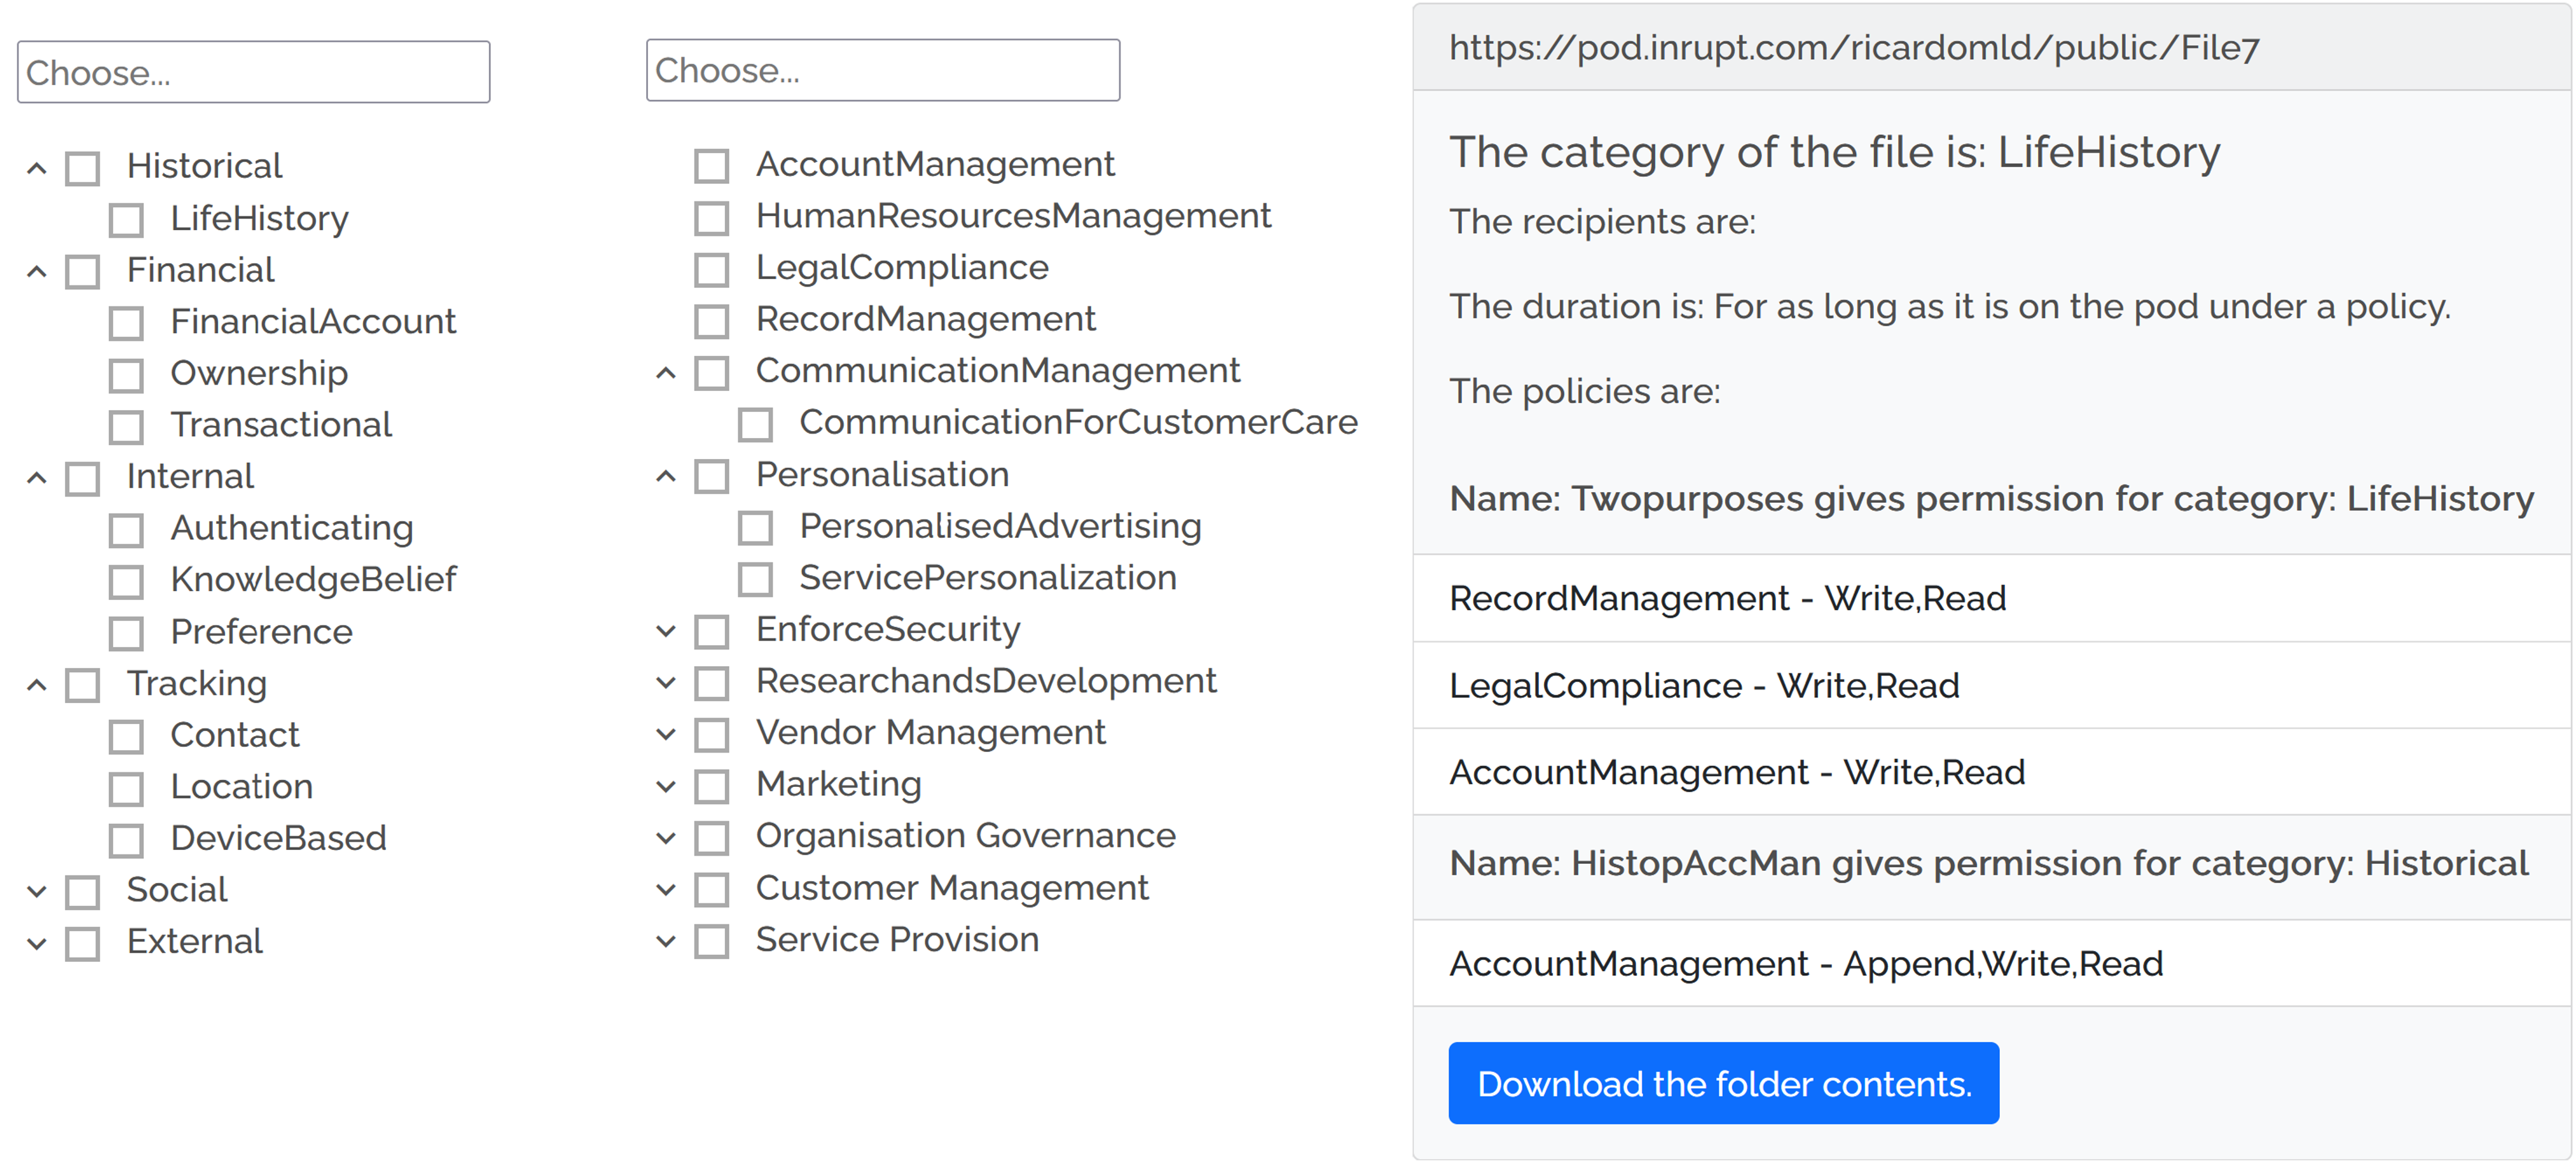
\includegraphics[width=0.8\linewidth]{figures//chapter-6/right-app.png}}
    \caption{Screenshot of an example Solid-based application that uses the implemented Right of Access API.}
    \label{fig:right-app}
\end{figure}

\paragraph{Maintenance, preservation, and future work}
The publication and archival of the developed work are performed according to the methodology described in Section~\ref{sec:code_preservation}.
Furthermore, the source code is hosted at \url{https://w3id.org/people/besteves/access-right/api} and \url{https://w3id.org/people/besteves/access-right/solid} (for the API and for the Solid app, respectively), under the MIT license.
These repositories can also be utilised by their users to suggest new features to be added to the work, as well as to document bugs through GitHub Issues.

In future developments, enhancements to the API could offer a more comprehensive response to a right of access request.
This would entail providing information on other data subject rights and clear details regarding data recipients, including their identities and contact information.
% Additionally, maintaining audit logs of the right's exercise could be implemented, with these logs stored in a dedicated container within the Pod for future reference.
Moreover, certain practical considerations have been overlooked.
For instance, it has been assumed that resources stored in the Pod under the influence of a policy can be automatically accessed through the API during their storage period.
This functionality could be expanded to accommodate new policy constraints, such as time-limited storage or periodicity constraints. 
Additionally, new parameters for filtering requested data could be incorporated into both the API and the Solid application.
